\chapter{Design of Experimental Platform}\label{ch:platform}

\section{Autopilot}

\section{Simulation}

\section{Airframe}

The aircraft used for this research was the Flitetest Spear \cite{flitetest}.  The Spear airframe was chosen for its endurance capability of greater than 45 minutes of flight time and it's large capacity fuselage.  The flying-wing architecture keeps the actuation requirement to a minimum of two servos by utilizing an elevon configuration.  

\begin{figure}[!h]
 \centering
  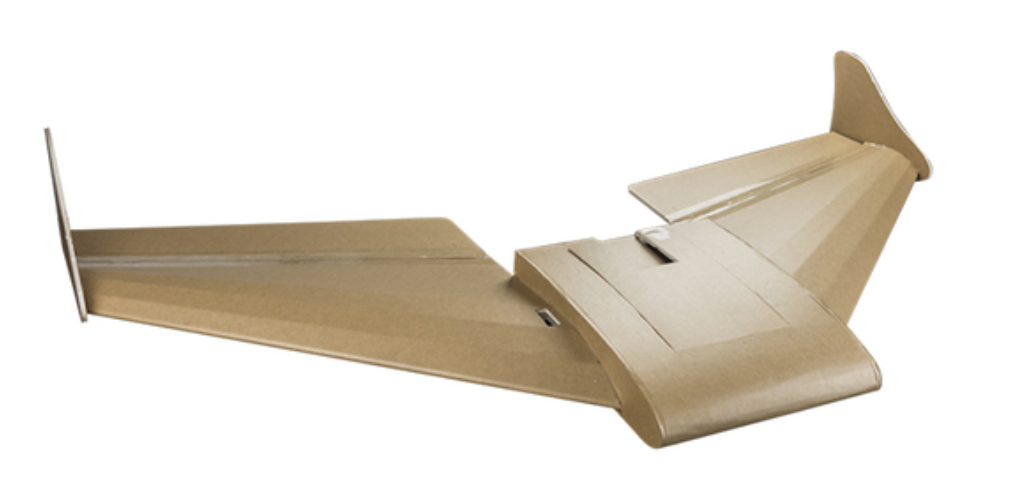
\includegraphics[width=0.65\textwidth]{spear.png}
  \caption{Spear Airframe}
  \label{fig:spear}
\end{figure}

The large blunt nose provides adequate space for two 2,200 mAh (12.6volts) lithium polymer batteries wired in parallel.  The remaining cargo space was used for accommodating the Pixhawk autopilot.

\begin{figure}[!h]
 \centering
  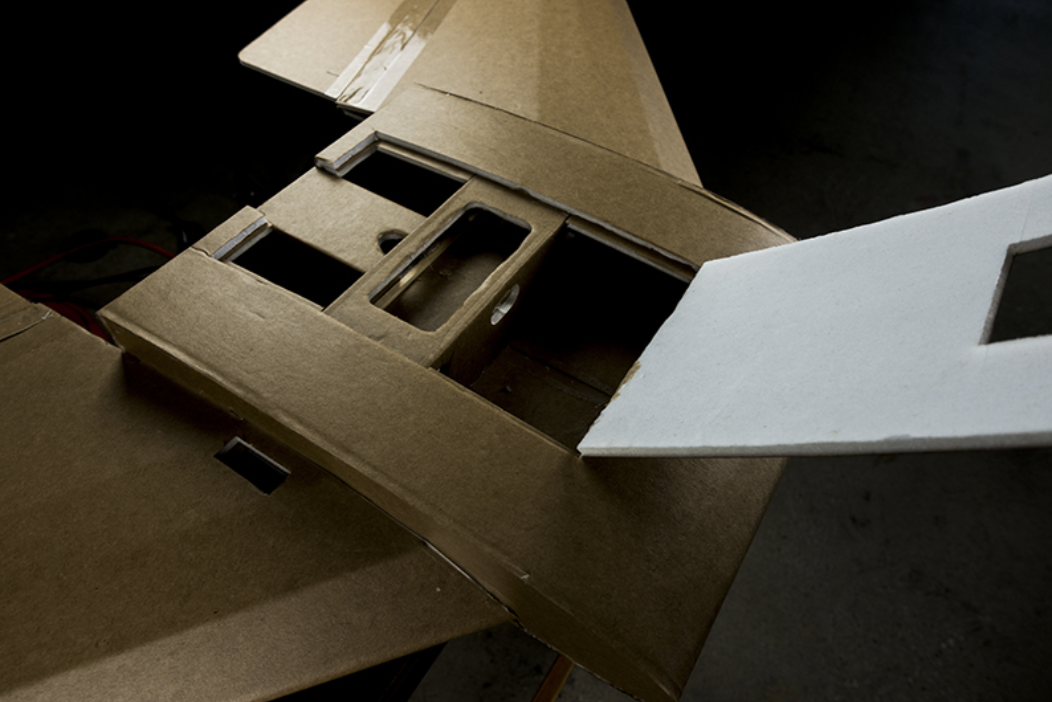
\includegraphics[width=0.50\textwidth]{spear_cargo.png}
  \caption{Spear Cargo Capacity}
  \label{fig:spear_cargo}
\end{figure}

This plane was constructed out of craft foam board.  The plans were downloaded from flitetest.com\cite{flitetest} and converted to CorelDraw vector files for use in a laser cutter.  These files were then cut out of four sheets of foam board using the laser cutter.  The wing halves were joined with standard box tape and hot-glue.  This provided a cheap and rapid construction process which was achievable under four hours of build time.

\begin{figure}[!h]
 \centering
  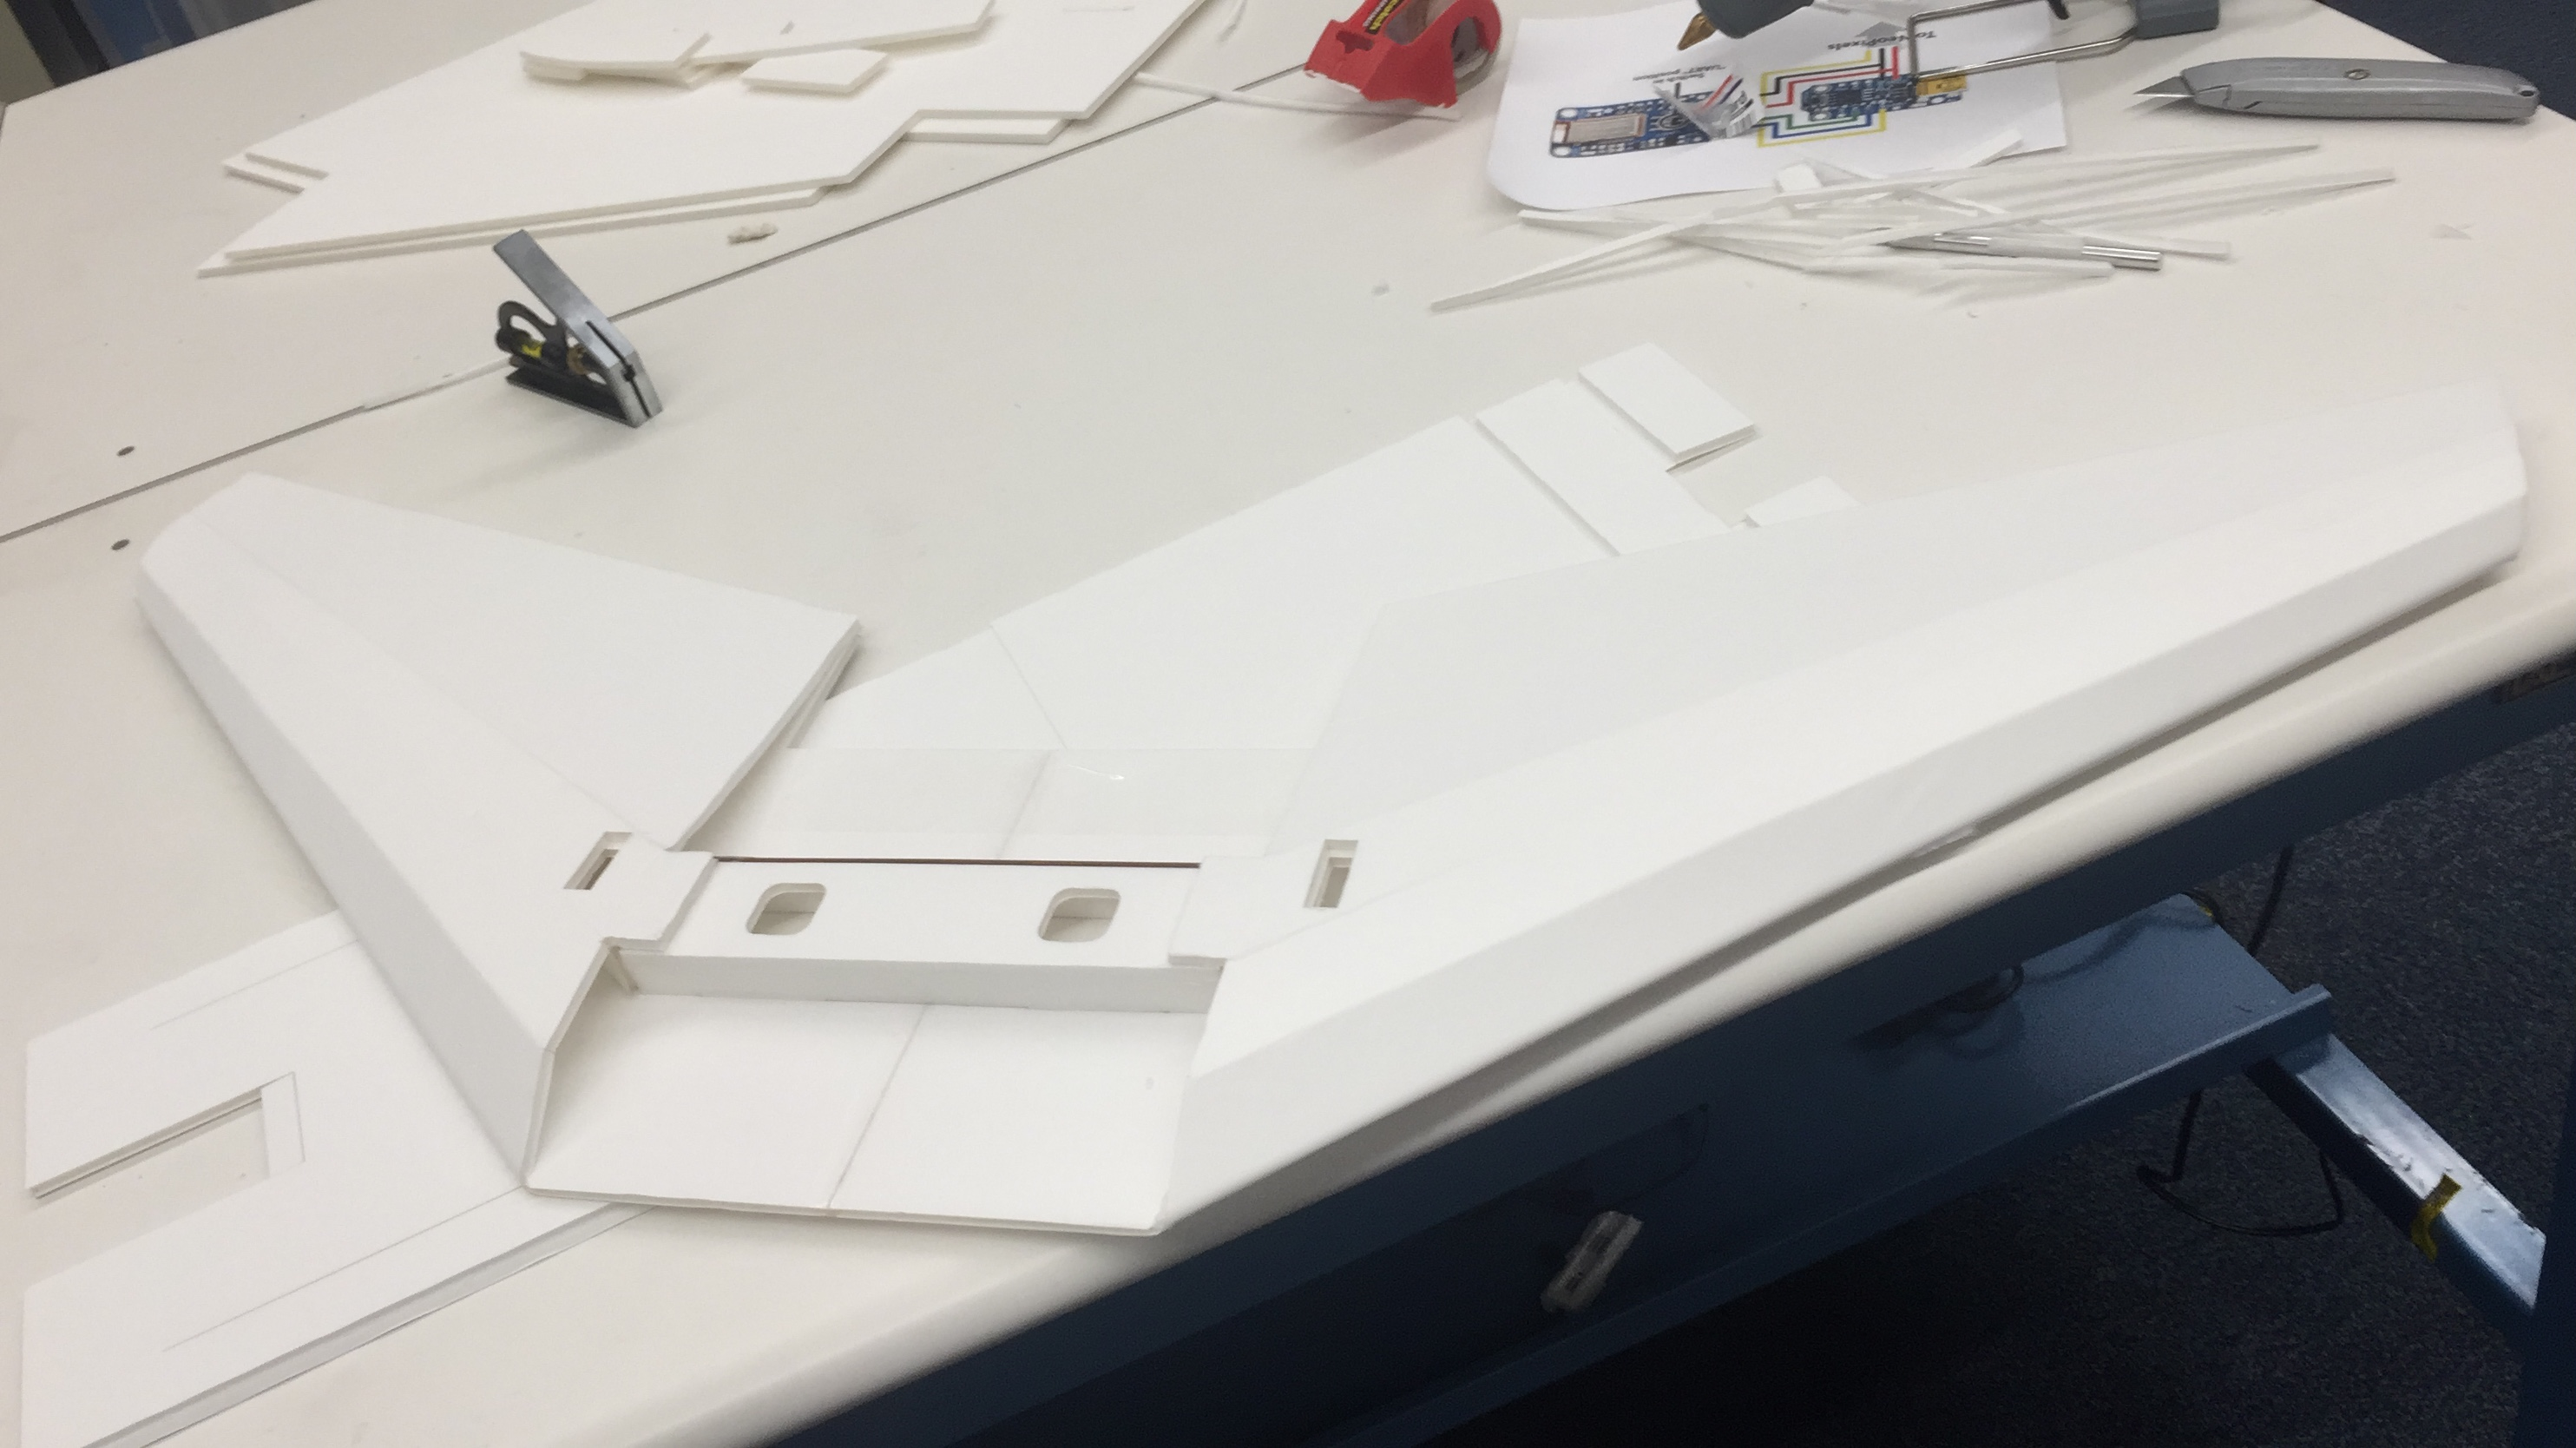
\includegraphics[width=0.65\textwidth]{spear_build.jpg}
  \caption{Spear Build Process}
  \label{fig:spear_build}
\end{figure}

The aircraft specifications are as follows:
\begin{itemize}
	\item Weight without battery: 1.45 lbs (658 g)
	\item Center of gravity: 3 – 3.5” (76 – 89 mm) in front of firewall
	\item Control surface throws: 16\degrees  deflection – Expo 30\%
	\item Wingspan: 41 inches (1041 mm)
	\item Recommended motor: 425 sized 1200 kv minimum
	\item Recommended prop: 9 x 4.5 CW (reverse) prop
	\item Recommended ESC: 30 amp minimum
	\item Recommended Battery: (2) 2200 mAH 12.6 volt minimum
	\item Recommended Servos: (2) 9 gram servos 
\end{itemize}



